\chapter{Results}\label{cha:results}

This section will present and discuss the results from the experiments presented in Section~\ref{sec:method-experiments}.
The modified SSD model presented in Section~\ref{sec:method-arch} is trained according to the training procedure given in Section~\ref{sec:method-exp-setup}.
Section~\ref{sec:results-baseline} presents the performance of the baseline model.
The results and discussion of the experiments pertaining to RQ1 and RQ2 are presented in Section~\ref{sec:results-simplification} and Section~\ref{sec:results-sharpness} respectively.
Threats to validity are provided in Section~\ref{sec:results-validity}.
Unless specified otherwise, all performance metrics given in this section are measured on the test split of the dataset.
For measuring mAP, the interpolation method specified in Equation~\ref{eq:average-precision} with an acceptance threshold of 0.5 IoU.

\section{Baseline model}\label{sec:results-baseline}
\begin{figure}[htbp]
    \centering
    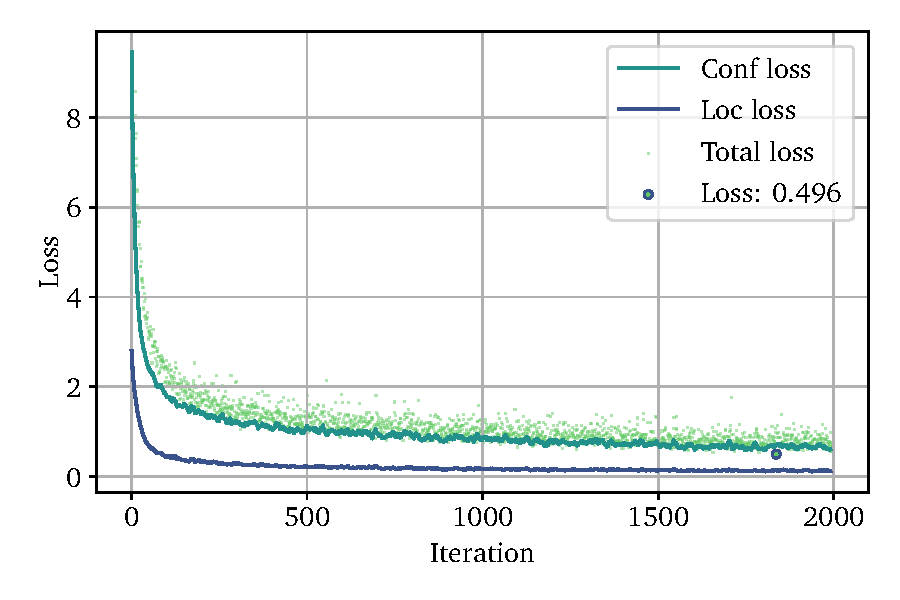
\includegraphics[width=0.7\textwidth]{figs/results/baseline/loss2.pdf}
    \caption[Baseline training procedure]{%
Training procedure for the baseline model over 2000 iterations.
The iterations given on the horizontal axis represent one forward-backpropagation run with one mini-batch, while the mini-batch averaged loss is given in the vertical axis.
The raw total loss values are shown with semi-transparent green points.
The solid lines show the moving means for the two individual loss components.
The green line shows the confidence loss component, while the blue line shows the localization loss component.
The mini-batch with the lowest total loss is annotated with a green circle and occurs after the 1800th iteration with a loss of 0.496.
    }\label{fig:method-baseline-loss}
  \end{figure}

The training procedure for the model is given in Figure~\ref{fig:method-baseline-loss} and exhibits a stochastic variation that is characteristic of mini-batch training.
The confidence loss component accounts for most of the total loss throughout the training process.
The components of the loss function (Equation~\ref{eq:loss}) are independent, meaning their ratio does not indicate a difference in performance at the two different tasks.
Regardless, the model does perform better at localization than classification.
Logically this follows from realizing that the pollen grains are all more easily distinguished from the background than they are to classify.
Therefore, the model can discriminate between background and pollen with relative ease but has a more challenging time classifying species.

\begin{figure}[htbp]
    \centering
    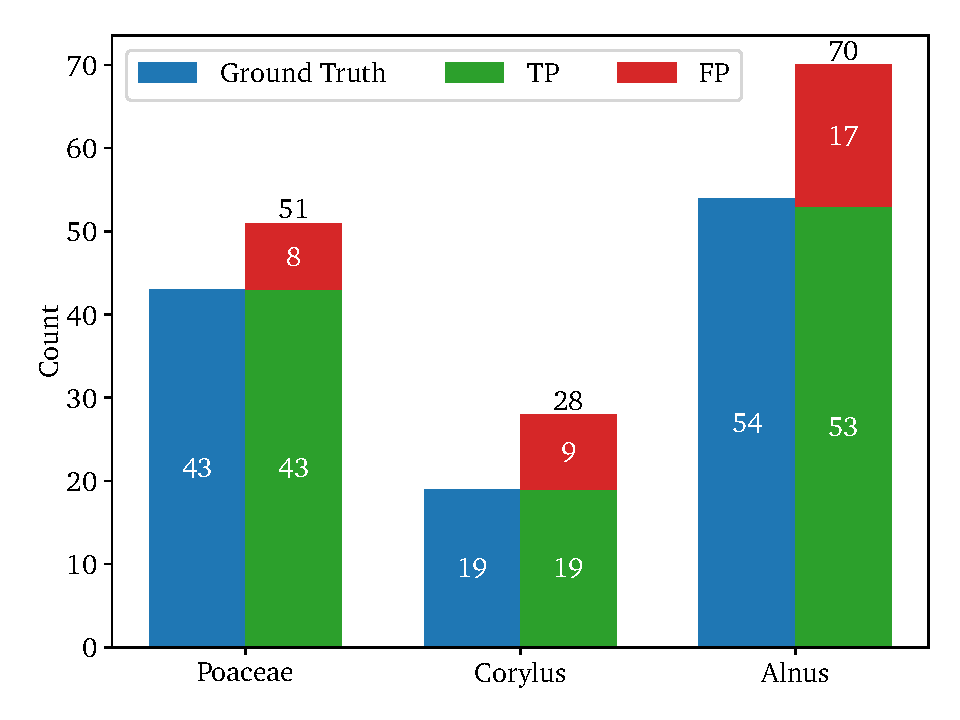
\includegraphics[width=0.7\textwidth]{figs/results/baseline/detections_test.pdf}
    \caption[Detections by type by class for the baseline on the test split] and an \(F_1\) score of \textbf{86.8\%}.
Looking at predictions overall, the recall is very high at 99.1\%, while precision is quite a bit lower at 77.2\%.
Figure~\ref{fig:results-baseline-detections} breaks down all the detections made; the main observation is that false-positive predictions are almost the only source of error.
37\% of false positives are spurious localization, i.e., an unlabeled entity is identified as a pollen grain.
These entities are either non-pollen particles or pollen grains from unlabeled species.
The remaining 63\% of false positives are misclassifications, i.e., the bounding box does correspond to a ground truth, but the class is incorrect.

\begin{figure}[htbp]
  \centering
  \begin{subfigure}[t]{0.4\textwidth}
    \centering
    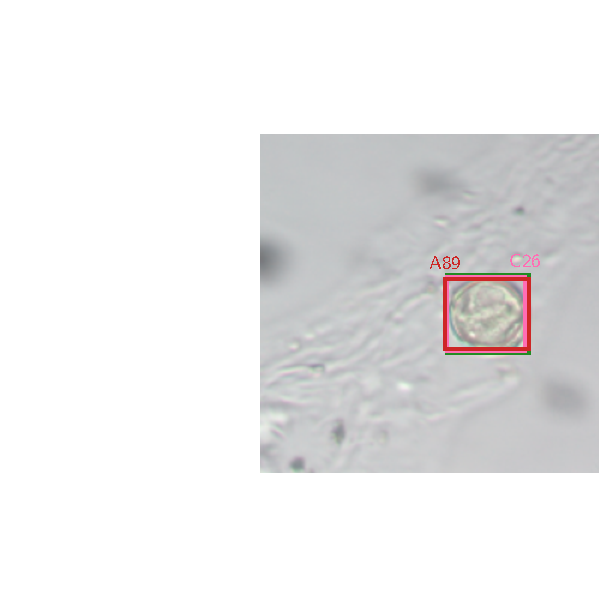
\includegraphics[width=\textwidth]{figs/results/baseline/Snap-408.pdf}
  \end{subfigure}%
  \hspace*{0.04\textwidth}
  \begin{subfigure}[t]{0.4\textwidth}
    \centering
    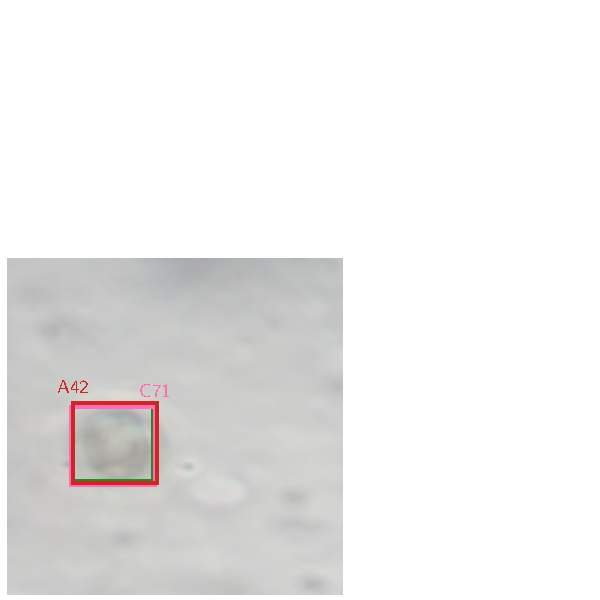
\includegraphics[width=\textwidth]{figs/results/baseline/Snap-028.pdf}
  \end{subfigure}
  \caption[Predictions showing TP overlapped by FP from different class]{Two predictions with GT in \textcolor{nicegreen}{green}, TP in \textcolor{red}{red}, and FP in \textcolor{nicepink}{pink}.
The labels give the first letter of the class and the prediction confidence in the range [0,100].
All TP labels are placed at the NW corner of the bounding box.
The FP labels are placed at the other three corners according to class.
In the left image, an FP box is predicted with lower confidence than the TP\@.
In the right image, the FP Corylus prediction has higher confidence than the TP Alnus prediction.}\label{fig:results-overlapping-predictions}
\end{figure}

Figure~\ref{fig:results-overlapping-predictions} shows two test samples containing overlapping true and false-positive predictions.
This is due to the NMS filtering algorithm being run for each class independently, which causes double predictions in cases where predictions for multiple classes are produced for the same pollen grain.

A remedy was implemented and tested where NMS was applied to all detections after the initial per-class NMS\@.
The results from this were ambiguous; The precision did improve due to the decreased number of FP predictions, but the decrease in TP predictions caused a similar decrease in recall.
In Figure~\ref{fig:results-overlapping-predictions} (right) for example, the correct prediction would get filtered out.

With the small number of classes in the dataset, the problem of double predictions is relatively small.
However, a larger dataset could suffer more from this issue when there are more classes that all share characteristics.
For the purposes of counting, it might not be preferable to prune these overlapping predictions but rather include and quantify the resulting overestimation as a part of the overall counting system.

\section{Model simplification}\label{sec:results-simplification}
The first two experiments aim to explore ways in which the computational complexity of the model can be reduced without sacrificing performance.
In the first experiment, the feature extraction network is substituted with lightweight alternatives.
In the second, the amount of default boxes is reduced by deactivating source feature maps.

\subsection{Feature extractor}
Table~\ref{tab:result-base-network} gives the results from training the network with different feature extraction networks.
As with the baseline, all the networks are designed for and trained on image classification datasets.
Larger networks, such as the deeper ResNet versions, could not be tested due to the memory limitations of the GPU\@.
There is a clear decrease in performance when using smaller networks, and we observe monotonically decreasing values for all performance metrics.

Interestingly, the recall remains almost unchanged, meaning that the model's ability to localize pollen grains is largely maintained.
The error is in the form of noise being added on top of the correct predictions.
The performance degradation is therefore primarily due to increased classification error, creating redundant, poor predictions.
A possible explanation for this is that localization, in terms of feature requirements, only requires the model to learn simple features relating to the general shape and color of a pollen grain, while classification involves more complex features that the smaller networks are not able to capture.

This experiment helps reveal the apparent inequality between the two tasks that the model is learning, namely localization and classification.
Localization seems to be a much easier task to learn, given how invariant the model is to the changing extractor while seeing a markedly higher degradation in classification.

\begin{table}[htbp]\centering
  \ra{1.3}
\caption[Performance by feature extraction network]{Summary of experimental results from testing various small feature extraction networks.
The localization score refers to the share of detection that correctly localizes a GT, regardless of class.
For each network, the number of trainable parameters for both the feature extractor and the whole model is given.}%
\label{tab:result-base-network}
\begin{tabular}{@{}lcrrrrcrr@{}}\toprule
  Network & \phantom{a} & \multicolumn{4}{c}{Performance} & \phantom{ab}&  \multicolumn{2}{c}{Parameters} \\
  \cmidrule{3-6} \cmidrule{8-9}
        &&  mAP &  Precision &  Recall &  Loc. &&  Extractor   & Total \\
  \midrule
     ResNet 34 && 95.2 &      82.7  &   99.1  & 95.0  &&  \num{8.2e6} & \num{1.2e7} \\
     ResNet 18 && 92.6 &      81.9  &   97.4  & 92.8  &&  \num{2.8e6} & \num{6.7e6} \\
  MobileNet V2 && 90.4 &      67.9  &   98.3  & 86.3  &&  \num{1.3e5} & \num{9.6e5} \\
  \bottomrule
\end{tabular}
\end{table}

\subsection{Layer activation}
In the next experiment, parts of the extra structure (shown as arrows in Figure~\ref{fig:model}), responsible for generating the detections as various scales are deactivated.
The results are given in Table~\ref{tab:result-layer-deactivated} and do not point towards any strong trend.
The last three layers of the model are larger than almost all grains in the dataset, and even with cropping, it is likely that their predictions do not contribute to the loss because the default boxes they encode rarely, if ever, get matched with a ground truth.
Their inclusion might result in parameters that do not get adequately trained, leading to those layers only producing noise instead of actual predictions.

For the models using only the first three layers, an improved mAP is observed, but the statistical significance is questionable.
However, this does call into question the importance of the larger feature maps and strengthens the initial belief that the SSD model can be simplified without compromising performance.

Other object detection tasks may also have certain differences in the distribution of size and shape of objects between classes.
The multiple layers then allow for specialization where some layers become better at detecting particular objects than others.
With pollen, there again is a much more uniform dataset where size differences between classes are negligible, which might also explain why there does not seem to exist any strong relationship between layer activation and performance.
This is compounded by the limited number of classes and could change if a larger, more diverse dataset was used.

\begin{table}[htbp]\centering
  \ra{1.1}
  \caption[Performance when deactivating source layers]{Summary of experimental results when deactivating various source layers.
  The source layers are ordered 1--6 with layer 1 being the most granular \(38\by38\) feature map.}%
  \label{tab:result-layer-deactivated}
\begin{tabular}{@{}llllllcrrr@{}}\toprule
  \multicolumn{6}{c}{Source layer activation} & \phantom{a} & \multicolumn{3}{c}{Performance}\\
  \cmidrule{1-6} \cmidrule{8-10}
  1 & 2 & 3 & 4 & 5 & 6 &&   mAP & Precision & Recall \\
  \midrule
  \ckm & \ckm & \ckm & \ckm & \ckm & \ckm && 95.3  & 84.6 & 99.1 \\
  \ckm & \ckm & \ckm & \ckm & \ckm &      && 95.5  & 77.4 & 99.1 \\
  \ckm & \ckm & \ckm & \ckm &      &      && 95.3  & 81.2 & 98.7 \\
  \ckm & \ckm & \ckm &      &      &      && \textbf{96.4}  & 79.3 & 99.1 \\
  \ckm & \ckm &      &      &      &      && 95.6  & 80.4 & 98.7 \\
  \ckm &      &      &      &      &      && 96.3  & 83.6 & 99.1 \\
       & \ckm &      &      &      &      && 95.7  & 85.5 & 99.1 \\
  \bottomrule
\end{tabular}
\end{table}

\section{Sharpness}\label{sec:results-sharpness}
The following two experiments look at how the sharpness of the ground truth data impacts model performance.
In the first experiment, the blurry grains are filtered from the training set to see the effect this has on the inferences made by the model.
In the second experiment, the dataset is split based on sharpness and measure the models' ability to make inferences across this sharpness boundary.

\subsection{Minimum training sharpness}\label{sec:results-minimum}
Our first experiment aims to explore how the sharpness of the training data affects the predictions that the model can make.
The results indicate that the model struggles with making inferences on grains with lower sharpness when such grains are filtered out of the training data.
Figure~\ref{fig:results-sharpness-gt} breaks down the ground truth labels into true positives and false negatives, which reveals that the model is failing to predict pollen grains that have a sharpness below the minimum sharpness of the training data.
\info{explain how this differs from cross sharpness}

Looking at the sharpness of the predictions made by the model, there is a corollary trend in the false positive predictions.
Figure~\ref{fig:results-sharpness-detections} shows that restricting the training data creates what seems to be a threshold, below which the model does not make predictions.
This shows that the model loses the ability to localize blurry pollen grains, becoming blind to their existence.
It seems clear that the features being learned from sharp images do not transfer to less sharp samples.

It is important to note that the sample size, especially in the case of false negatives, is relatively small, which weakens arguments made based on their distributions.
The observed pattern could also be described as a type of `overfitting' where the model will not generalize outside of the sharpness bound of the training data, and the implications this has for a hypothetical production system are unclear.

\begin{figure}[htbp]
  \centering
  \begin{subfigure}[t]{\textwidth}
    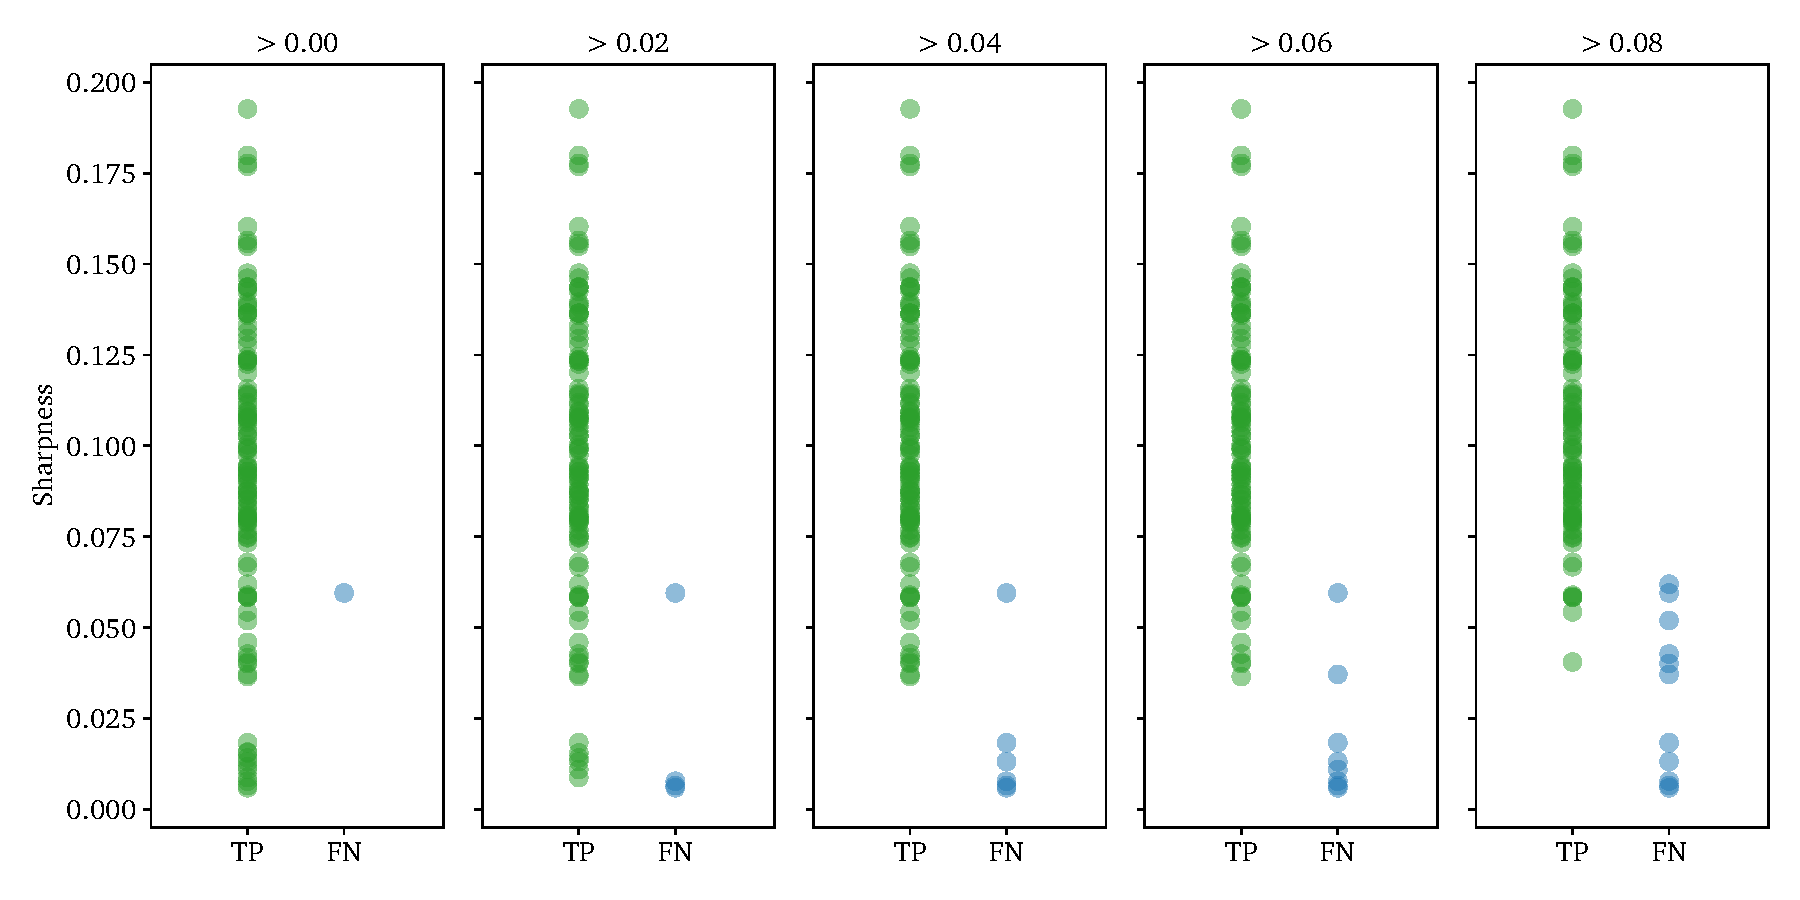
\includegraphics[width=\textwidth]{figs/results/sharpness/sharpness_TP_vs_FN.pdf}
    \subcaption{Sharpness distribution of \textit{ground truths} by prediction result in test split by minimum training sharpness}\label{fig:results-sharpness-gt}
  \end{subfigure}
  \begin{subfigure}[t]{\textwidth}
    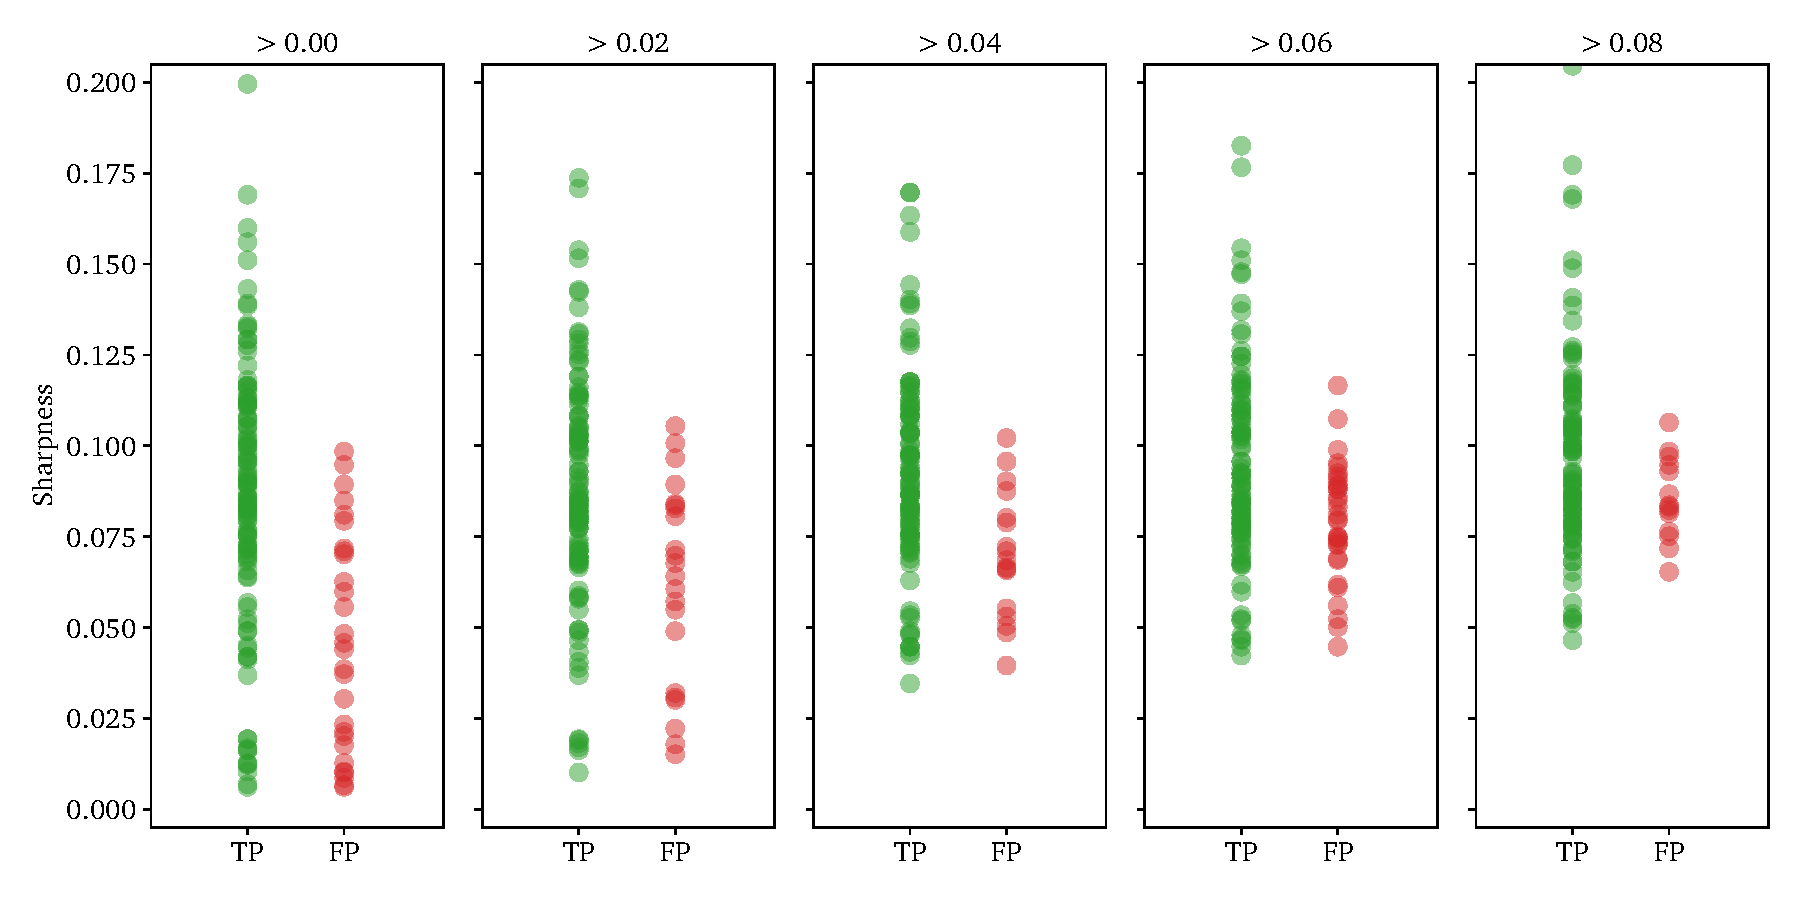
\includegraphics[width=\textwidth]{figs/results/sharpness/detection_sharpness_TP_vs_FP.pdf}
    \subcaption{Sharpness distribution of \textit{model predictions} by prediction result in test split by minimum training sharpness}\label{fig:results-sharpness-detections}
  \end{subfigure}
  \caption[Sharpness distribution of model predictions in test split by minimum training sharpness]{%
  Five experimental runs are shown, ground truth labels are filtered out of the training set by the sharpness requirement given in the plot header. In~\subref{fig:results-sharpness-gt}, sharpness is measured on original images using ground truth bounding boxes. In~\subref{fig:results-sharpness-detections}, sharpness is measured on the resampled \(300\by300\) pixel patches. This affects the scaling of the sharpness measure, and sharpness values from the two figures are therefore not directly comparable.
  }\label{fig:results-sharpness-minimum}
\end{figure}

\subsection{Cross-sharpness inference}
The final experiment aims to explore how well the model can generalize to a sharpness range that differs entirely from that of its training data.
Figure~\ref{fig:results-sharpness-inference} gives a summary of the experimental procedure.
As might be expected, the model performs best in the scenarios where it is trained and tested on grains in the same range of sharpness, and it performs worse when there is no overlap between test sharpness and training sharpness.

\begin{figure}[htbp]
  \centering
  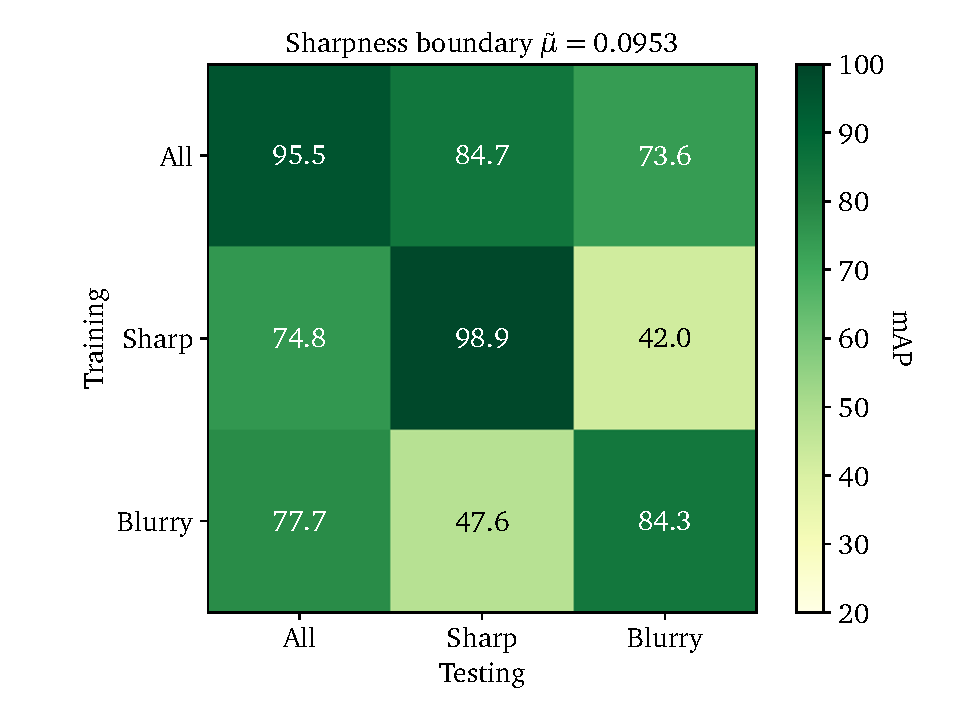
\includegraphics[width=0.9\textwidth]{figs/results/sharpness/confustion_balanced_test_map.pdf}
  \caption[mAP across sharpness boundary]{%
The confusion matrix shows the result from training and testing the model on three versions of the dataset.
The median sharpness value, \(\tilde{\mu}\), is used as a boundary and the dataset is divided into a sharp (\(>\tilde{\mu}\)) and a blurry (\(<\tilde{\mu}\)) data set.
The same training/testing split is still used.
The horizontal axis denotes the version of the dataset used when computing mAP, while the vertical axis denotes the dataset used when testing.
Two quadrants stand out with significantly lower scores; these represent the scenarios where the model is trained on either the sharp or the blurry data and tested on the opposite.
  }\label{fig:results-sharpness-inference}
\end{figure}

Interestingly, the model responds differently to being trained on only blurry data (the `blurry' model) than being trained on only sharp data (the `sharp' model).
Seemingly, the blurry model outperforms the sharp model both when tested on the whole dataset and when tested across the sharpness boundary.
It seems as though the same kind of overfitting is not taking place, and the blurry model is learning features from the blurry data that it can use to detect sharp pollen grains.

\begin{figure}[htbp]
  \centering
  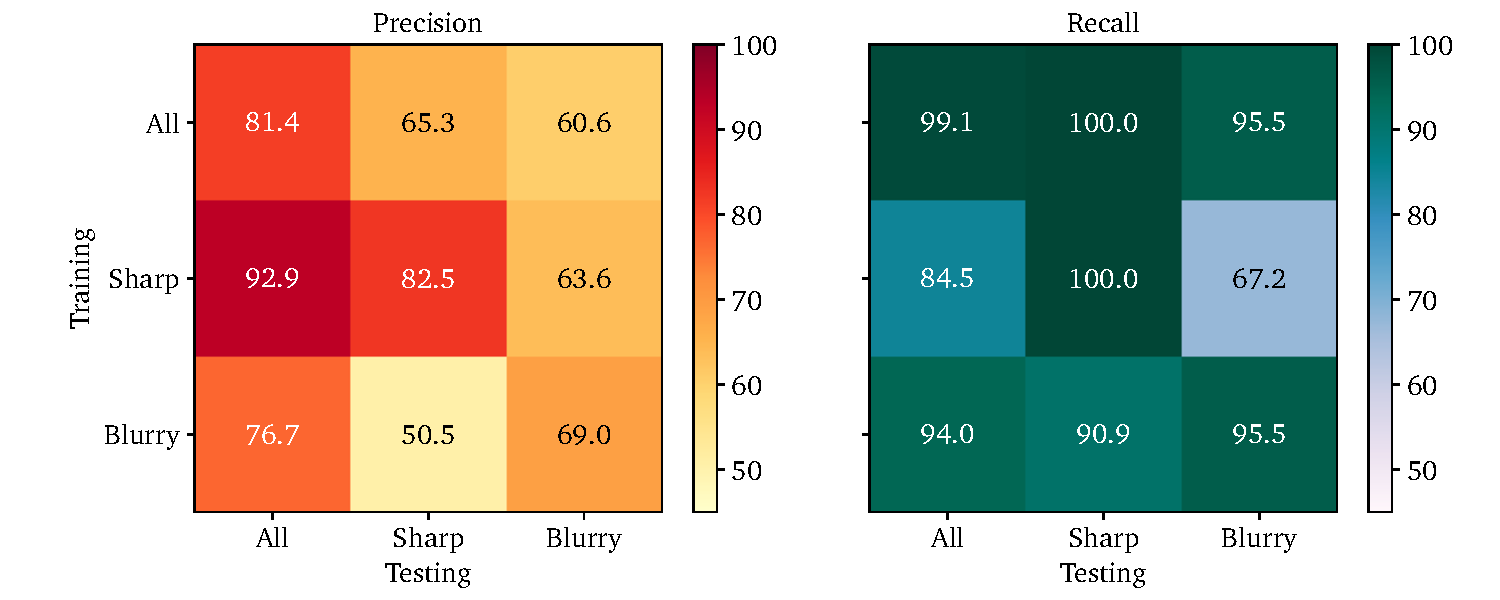
\includegraphics[width=\textwidth]{figs/results/sharpness/confustion_balanced_test_dual.pdf}
  \caption[Precision \& Recall across sharpness boundary]{%
Breakdown of precision and recall values for cross-sharpness training. See Figure~\ref{fig:results-sharpness-inference} for detailed explanation.
  }\label{fig:results-sharpness-pr-rec}
\end{figure}

Figure~\ref{fig:results-sharpness-pr-rec} shows the precision and recall values separately and gives more insight into the differences between the two models.
Looking at recall, the sharp model performs worse than the blurry model when tested across the sharpness boundary.
Looking at precision, the opposite is true, however to a lesser degree.
This shows that the models are underperforming for different reasons.
The sharp model maintains its classification performance but fails to localize pollen grains that are too blurry. In contrast, the blurry model maintains its ability to localize all pollen grains but struggles with classifying them.

Similar to how simplifying the feature extractor leads to worse classification performance while localization is maintained, the same response is seen when the granular features are smoothed out by blur.
What this implies for further development of this system is difficult to say and depends on the requirements of the system.
In a scenario where the model only needs to work on sharp data, excluding blurry data could improve overall performance.
However, one can easily imagine a system that could benefit from being able to localize outside the current focus plane, e.g., in a search-based system that explores a slide live, the model could localize a blurry grain and refocus the microscope to classify it.

\begin{figure}[htbp]
  \centering
  \begin{subfigure}[t]{0.35\textwidth}
    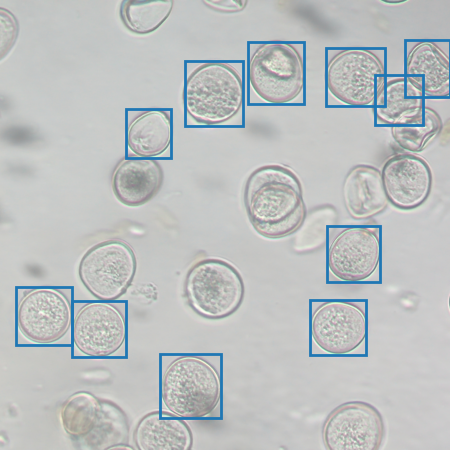
\includegraphics[width=\textwidth]{figs/results/sharpness/Snap-242-sharp.png}
    \subcaption{Sharp labels}\label{fig:results-sharpness-sharp}
  \end{subfigure}
  \hspace*{0.4em}
  \begin{subfigure}[t]{0.35\textwidth}
    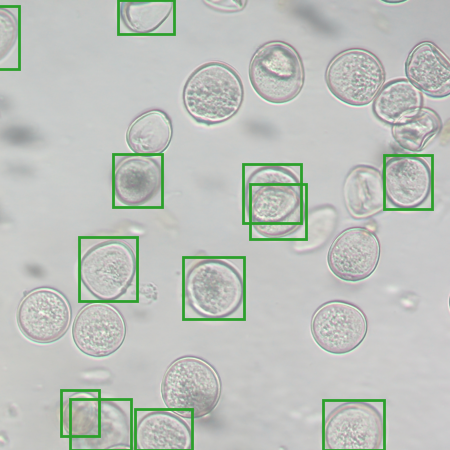
\includegraphics[width=\textwidth]{figs/results/sharpness/Snap-242-blurry.png}
    \subcaption{Blurry labels}\label{fig:results-sharpness-blurry}
  \end{subfigure}
  \caption[Data sample showing split between sharp and blurry data]{%
Sample from the dataset. Ground truths in the sharp partition are drawn in \textcolor{poaceae}{blue}, while the blurry are drawn in \textcolor{alnus}{green}.
  }\label{fig:results-sharp-gt}
\end{figure}

While it seems to follow logically from the presence of more granular and detailed features in sharp data that the sharp model is more precise than its blurry counterpart, it is less obvious why it seemingly loses all ability to localize blurry grains.
One possible explanation becomes apparent when looking not at the labeled data but at everything else the model is asked to ignore.

As a result of the data collection procedure, where at least one pollen grain is entirely in focus in every sample, the sharpest object in any given sample is always a pollen grain.
Figure~\ref{fig:results-sharp-gt} shows an example of the split, and reveals that all in-focus objects are labeled ground truths.
This trend holds over the entire dataset, where almost every object that appears in focus is a labeled ground truth.
The inverse assumption that everything out of focus is not a ground truth does not hold, except in the sharp training split.
So while the sharp model can rely almost entirely on the presence of sharp features when learning `what is a pollen grain?', the blurry and baseline models must also learn to differentiate between out of focus pollen grains and out of focus background.

The boundary value is set to the median sharpness value over the total training split.
This was done to give each model the same number of ground truths.
While this is a valid decision, looking at Figure~\ref{fig:results-sharp-gt}, many pollen grains in the blurry category seem pretty sharp to the naked eye.
With a larger dataset, it would be preferable to run this experiment with multiple splits.
The optimal sharpness distribution remains unknown, although evidence has been presented to support the claim that excluding blurry data causes the model to fixate on only the sharp features in images.
\info[inline]{Summarize results. 1--2 par.}

\section{Threats to Validity}\label{sec:results-validity}
\info[inline]{Move to future work such that each threat has an accompanying suggestion for an improvement}
Throughout the preceding Sections, the results and weaknesses of the experiments have been discussed.
This section highlights more general threats to the validity of the project as a whole.

\subsection{Number of classes}
The size of the dataset could pose a threat to the external validity of the model's performance.
The results show that the model performs better at localization than at classification in a dataset containing three distinct classes within a domain where most classes share similar features.
It is unknown how the model would perform with a dataset containing more classes and if it could maintain its ability to label classes correctly.
Therefore, it cannot be concluded that the model would perform at a similar level of precision in datasets with more classes.

\subsection{Sharpness measure}
The results assume a link between perceived sharpness and focal planes in the sample images without a direct correlation being shown.
This perceived sharpness is used to validate the sharpness measure, which in turn is used to analyze the model in relation to data sharpness.
To an extent, this assumption does hold; when the focal plane lies above or below a pollen grain, perceived sharpness changes with the focal plane.
However, on a more granular level, how the sharpness measure corresponds to the location of the focal plane when it lies within a pollen grain is less clear.
From observation, maximum sharpness does seem to occur at the center of the pollen grain when the diameter of the grain is largest.

\subsection{Training procedure}
The short training time allows for many experimental runs, but fine-tuning hyperparameters for every configuration was outside time constraints.
This could mean that certain runs are offered an advantage which would cause systematic errors in the results.

The number of samples overall also contributes to very volatile performance results.
Due to the limited number of ground truths in the test split, small differences in the models significantly impact measured performance.
